% 
% Annual Cognitive Science Conference
% Sample LaTeX Paper -- Proceedings Format
% 

% Original : Ashwin Ram (ashwin@cc.gatech.edu)       04/01/1994
% Modified : Johanna Moore (jmoore@cs.pitt.edu)      03/17/1995
% Modified : David Noelle (noelle@ucsd.edu)          03/15/1996
% Modified : Pat Langley (langley@cs.stanford.edu)   01/26/1997
% Latex2e corrections by Ramin Charles Nakisa        01/28/1997 
% Modified : Tina Eliassi-Rad (eliassi@cs.wisc.edu)  01/31/1998
% Modified : Trisha Yannuzzi (trisha@ircs.upenn.edu) 12/28/1999 (in process)
% Modified : Mary Ellen Foster (M.E.Foster@ed.ac.uk) 12/11/2000
% Modified : Ken Forbus                              01/23/2004
% Modified : Eli M. Silk (esilk@pitt.edu)            05/24/2005
% Modified : Niels Taatgen (taatgen@cmu.edu)         10/24/2006
% Modified : David Noelle (dnoelle@ucmerced.edu)     11/19/2014
% Modified : Roger Levy (rplevy@mit.edu)     12/31/2018



%% Change "letterpaper" in the following line to "a4paper" if you must.

\documentclass[10pt,letterpaper]{article}

\usepackage{cogsci}

% \cogscifinalcopy % Uncomment this line for the final submission 

% \usepackage{times}
% \cogscifinalcopy % Uncomment this line for the final submission 


\usepackage{pslatex}
\usepackage{apacite}
\usepackage{float} % Roger Levy added this and changed figure/table
                   % placement to [H] for conformity to Word template,
                   % though floating tables and figures to top is
                   % still generally recommended!

%\usepackage[none]{hyphenat} % Sometimes it can be useful to turn off
%hyphenation for purposes such as spell checking of the resulting
%PDF.  Uncomment this block to turn off hyphenation.
\usepackage{graphicx}
\usepackage{amsmath}
\usepackage{amssymb}
\usepackage{booktabs}
\usepackage{xcolor}
\usepackage{lipsum}
\usepackage{multicol}
\usepackage{multirow}
\usepackage{epigraph}
\usepackage{natbib}
\usepackage[T1]{fontenc}
% \usepackage{natbib}

\DeclareSymbolFont{letters}     {OML}{cmm} {m}{it}
\DeclareMathAlphabet\mathcal{OMS}{cmsy}{m}{n}
\SetMathAlphabet\mathcal{bold}{OMS}{cmsy}{b}{n}

\definecolor{yello}{HTML}{ffb677}
\definecolor{blu}{HTML}{005082}
\definecolor{purpl}{HTML}{726a95}
\definecolor{orang}{HTML}{ff9a76}
\definecolor{tealish}{HTML}{1aa6b7}

\newcommand\BibTeX{B\textsc{ib}\TeX}

\newcommand{\ake}[1]{\textcolor{blue}{$_{AE}$[#1]}}
\newcommand{\km}[1]{\textcolor{purple}{$_{KM}$[#1]}}
\newcommand{\todo}[1]{\textcolor{purple}{$_{todo}$[#1]}}
\newcommand{\new}[1]{\textcolor{blu}{#1}}
\newcommand{\blank}{$\rule{0.6cm}{0.15mm}$}

\newcommand{\pp}{\mathcal{P}}
\newcommand{\cc}{\mathcal{C}}
\newcommand{\sss}{\mathcal{S}}
\newcommand{\mask}{\textsc{[mask]}}
\newcommand{\cls}{\textsc{[cls]}}
\newcommand{\sep}{\textsc{[sep]}}


% \newcommand{\induction}[2]{% \logicarg{<premise>}{<conclusion>}
% \begin{equation}
%     \begin{tabular}{@{}l@{}}
%         #1 \\ \midrule #2
%     \end{tabular}%
% \end{equation}
% %   \begin{tabular}{@{}l@{}}
% %     #1 \\ \midrule #2
% %   \end{tabular}%
% }


\setlength\titlebox{4.5cm}
% You can expand the titlebox if you need extra space
% to show all the authors. Please do not make the titlebox
% smaller than 4.5cm (the original size).
%%If you do, we reserve the right to require you to change it back in
%%the camera-ready version, which could interfere with the timely
%%appearance of your paper in the Proceedings.

% \raggedbottom
\setlength{\parskip}{0pt}
\makeatletter
\renewcommand{\paragraph}{%
  \@startsection{paragraph}{4}%
  {\z@}{1ex \@plus 1ex \@minus .2ex}{-1em}%
  {\normalfont\normalsize\bfseries}%
}
\makeatother

\title{A Property Induction Framework for Neural Language Models}
 
\author{
{\large \bf Kanishka Misra$^{\spadesuit}$ (kmisra@purdue.edu)\\
\large \bf Allyson Ettinger$^{\clubsuit}$ (aettinger@uchicago.edu) \\
\large \bf Julia Taylor Rayz$^{\spadesuit}$ (jtaylor1@purdue.edu)} \\
  $^{\spadesuit}$Department of Computer and Information Technology,
  Purdue University, IN, USA \\
  $^{\clubsuit}$Department of Linguistics, University of Chicago, IL, USA
}

\begin{document}

\maketitle


\begin{abstract}
Include no author information in the initial submission, to facilitate
blind review.  The abstract should be one paragraph, indented 1/8~inch on both sides,
in 9~point font with single spacing. The heading ``{\bf Abstract}''
should be 10~point, bold, centered, with one line of space below
it. This one-paragraph abstract section is required only for standard
six page proceedings papers. Following the abstract should be a blank
line, followed by the header ``{\bf Keywords:}'' and a list of
descriptive keywords separated by semicolons, all in 9~point font, as
shown below.

\textbf{Keywords:} 
add your choice of indexing terms or keywords; kindly use a
semicolon; between each term
\end{abstract}


\section{Introduction}
\todo{Conceptual knowledge from text. Success of LMs in several tasks requiring access to complex reasoning and high level cognition. LMs are therefore a candidate to study the claims made in first few lines \citep{lupyan2019words}.}
\todo{In this paper, we develop a framework that weighs in on the debate by studying conceptual knowledge in LMs. Specifically, we focus on Induction, definition, while IR can be any non-DR, we focus on knowledge about mental representations of everyday knowledge and reasoning (concepts), the set of objects or items they pick out (categories), and their properties. Inductions involving these things is often called property induction \citep{}.}
% \todo{Definition of property induction, its prevalence in the study of semantic cognition.}
% Inductive reasoning, or Induction is defined as the use of existing knowledge to make inferences about novel situations \citep{hayes2018inductive}.
% It fundamentally differs from deductive reasoning in that it is a form of reasoning where the conclusions do not deductively follow from the premise \citep{chater2011inductive, kemp2014taxonomy}.
% Instead, the reasoner must fundamentally go beyond the available data to make conclusions that are likely but not certain \citep{kemp2009structured, hayes2018inductive}. 
% % Under such an interpretation, induction can be construed as probabilistic reasoning.
% For example, on encountering a new property attributed to the concept \textsc{robin}, one might generalize (or project) it to the entire \textsc{bird} category \citep{osherson1990category}.
% The general principles of induction can be applied to a myriad of different problems in the study of cognition.
% In this paper, we consider a subset of the universe of inductive problems \citep{kemp2014taxonomy} that deal with one's knowledge of concepts, categories, and properties, often collectively called \textbf{category-based induction} \citep{osherson1990category} or \textbf{property induction} \citep{gelman1986categories}.

% Meanwhile, 
% \todo{Inductive reasoning as being essential for the study of human cognition. Carey's work, Rogers and McClelland, touchstone phenomena by osherson highlighting the inductive bias of humans. Meanwhile, unprecedented computational advances in NLP have lead to NLMs, impressive model behavior, even on tasks requiring access to high level cognition. To what extent can conceptual knowledge be acquired by sole exposure from text in a manner that it can be \textit{used} in the correct context?}
% more on usage -- most studies compare similarities directly, induction principally involves \textit{making statistical decisions} based on similarities, and assessing the degree of correspondence between the generalizations made by LMs and Humans.
% Privileged status of taxonomies in the study of semantic cognition.
% Taxonomies have a privileged status in the study of concepts and semantic cognition in general -- from inquiries into the nature of semantic memory \citep{collins1969retrieval} to studies on graded, typicality effects \citep{rosch1975cognitive} and the `basic-level' \citep{rosch1976basic, rosch1978cognition}, to the word learning research by \citet{xu2007word}, \textit{inter alia}.
% In the context of property induction, \citet{gelman1986categories} were one of the first ones to observe the role of taxonomic relations emerge in patterns of induction in children and adults. 
% In their experiments, \citeauthor{gelman1986categories} first displayed a picture of a flamingo to their subjects and informed them that it had a ``right aortic arch,'' then displayed a picture of a bat and told them that it had a ``left aortic arch.'' 
% The subjects were then shown a picture of a blackbird (that visually resembled the bat more than it did the flamingo), and were asked whether it had a right or a left aortic arch. The subjects attributed the ``right aortic arch'' to the blackbird, indicating a \textit{taxonomic bias} in their inductive judgments.
% Building on research by \citet{gelman1986categories},
% \citet{osherson1990category} use the notion of \textit{similarity} to describe their observations in a landmark paper, that documented 13 separate phenomena related to taxonomies, that drove induction in humans.
% \todo{Induction as reasoning beyond the available data -- by using background knowledge. Humans reason inductively on a daily basis, induction is therefore prevalent in the study of semantic cognition.}
% \todo{Progress in NLP -- language models that demonstrate impressive performance on a range of tasks requiring access to high level cognition!}

\todo{Potential of property induction to reveal how people and LMs generalize knowledge beyond available data.}

\todo{we propose a framework for performing property induction with LMs to shed light on blah blah, how we use it to test two qualitative patterns prevalent in human induction literature.}
\todo{findings}

% \section{Related Work}
% \todo{this probably shouldn't be too detailed}
% \subsection{Computational Models of Property Induction}

% \subsubsection{Bayesian Models}

% \subsubsection{Connectionist Models}
% \section{Inductive Inferences in \citet{rogers2004semantic}}
\section{Connectionist Approaches to Property Induction}
\todo{LMs are basically early connectionist models on steroids, and exclusively learn from statistics of language data.}
\todo{describe R\&M, main task, how they operationalize induction (as \textit{backpropagation})} have 

\todo{Alternative research program that uses bayesian models, different in philosophy but could be different levels of cognitive models \citep{}, non-trivial to shed light on how language might contribute to semantic knowledge using this approach.}

\section{The Framework}
\todo{Alternatives and their pitfalls, Desiderata}
\subsection{Property Judgment Stage}
\subsection{Induction Stage}
% \km{(backpropagation is desirable -- straightforward interpretation as integration of new knowledge by updating model representations that are then used to inform how the new property will generalize. It also  lets us directly quantify the level of acceptance of the new information in terms of the the loss after each backpropagation step.)}

% Every instance of a property induction experiment consists of the application of a novel property to a set of one or more premise concepts (collectively denoted as the adaptation set, $\adaptation \subset \concepts$), and to a set of conclusion concepts (collectively denoted as the generalization set, $\generalization \subset \concepts$).
% OLD: An instance of a property induction experiment involves first associating a novel property to a set of one or more premise concepts (collectively denoted as the adaptation set, $\adaptation \subset \concepts$), and then assessing how likely does it generalize to a set of conclusion concepts (collectively denoted as the generalization set, $\generalization \subset \concepts$).
% OLD: This results in two sets of one or more sentences, each corresponding to the premise and the conclusion of a single property induction instance.
% The premise and conclusion of each instance are represented as sentences.
% POTENTIALLY better placed in Intro: 
%In brief, we construct premise and conclusion sentences based on concepts concerning a given induction phenomena we wish to study, and pair them with the desired novel property. 
% We operationalize induction as ``domain adaptation'' where the model is adapted to classify the premise sentences as true, using standard \textit{backpropagation}, after which the model is frozen and is then queried on the conclusion sentences to measure how likely is the property applicable to the conclusion concepts.
% Each instance of property induction involves a set of concepts that are relevant to overarching inductive behavior to be assessed. 
% For instance, \cref{arg:example} describes the generalization of a property from a subordinate to the entire \textsc{bird} category.
% We denote the set of relevant concepts as the source set $\source$. $\source$ is further differentiated into two sets: the adaptation set $\adaptation$, and the generalization set $\generalization$. 
% Concepts in $\adaptation$ and $\generalization$ are each paired with the novel property involved to from premise and conclusion sentences, respectively.
% Depending on the specific inductive phenomena being simulated, 

\section{Property Judgment Experiments}
\subsection{Data} \todo{pitfalls of using property norms directly -- absence of evidence vs evidence of absence, stereotypes, proper nouns, subjective properties}
\todo{Solution: manual annotation}
\subsection{Models}
\subsection{Training}
\subsection{Results}

\section{Investigating Inductive Generalizations}
\subsection{Premise Monotonicity}
\paragraph{Stimuli Generation}
\subsection{Conclusion Specificity}
\paragraph{Stimuli Generation}


\section{Discussion}
% We observe that while the patterns of generalization in BERT-large roughly remained the same, there were notable changes in those of ALBERT-xxl and RoBERTa-large. Specifically, the relative preference to generalize between ``Within-category'' and ``Outside-category'' decreased for ALBERT-xxl, and increased for RoBERTa-large.
% \km{Empirically, property-overlaps had a significant positive but weak effect for }

% Overall, there is still a preference towards
% \km{Shown in \Cref{fig:taxonomicresults}B. We see than albert decreases, bert almost remains the same, and roberta increases slightly. Suggests that at least }
% \km{Inductive generalizations are often studied using novel properties. So when a model is given a novel property, there could be a number of hypotheses one might have about how it generalizes. Consider the example when the model is given a new property ``\textit{can fep}'' that is associated with \textsc{cat}. One hypothesis could be that the model uses representational similarity to project new properties -- i.e., if \textsc{dog} is close to \textsc{cat} in the vector space of the model, then the model will assign high probability to ``\textit{a dog can fep}.'' Another hypothesis could focus on testing whether the model has learned category-membership, and may prefer generalizing to members of the same category }
% As a case-study, we will focus on inductive generalizations made on the basis of taxonomic relations between concepts and ask whether the models use knowledge of category-membership to make project newly provided properties.
% For instance, when given that a new property, ``\textit{can fep}'' is associated with \textsc{cat}, do models prefer generalizing it to other mammals (\textsc{dog, cow, buffalo}, \dots) over a set of other animal concepts (\textsc{salmon, robin, ant}, \dots)?

% inductive generalizations made on the basis of taxonomic relations between concepts, and ask the extent to which LM representations support generalization of new properties associated with a given set of concepts (\textsc{robin, sparrow, eagle}) to concepts \km{in X versus concepts }

% Taxonomies have a privileged status in the study of concepts and semantic cognition in general -- from inquiries into the nature of semantic memory \citep{collins1969retrieval} to studies on graded, typicality effects \citep{rosch1975cognitive} and the `basic-level' \citep{rosch1976basic, rosch1978cognition}, to the word learning research by \citet{xu2007word}, etc.
% In the context of property induction, \citet{gelman1986categories} were one of the first ones to observe the role of taxonomic relations emerge in patterns of induction in children and adults. 
% In their experiments, \citeauthor{gelman1986categories} first displayed a picture of a flamingo to their subjects and informed them that it had a ``right aortic arch,'' then displayed a picture of a bat and told them that it had a ``left aortic arch.'' 
% The subjects were then shown a picture of a blackbird (that visually resembled the bat more than it did the flamingo), and were asked whether it had a right or a left aortic arch. The subjects attributed the ``right aortic arch'' to the blackbird, indicating a \textit{taxonomic bias} in their inductive judgments.
% Building on research by \citet{gelman1986categories},
% \citet{osherson1990category} documented 13 separate induction phenomena related to taxonomies in their landmark paper.
% \km{Prevalence of taxonomic generalization in investigations of human generalization, various phenomena assimilated by induction researchers.}
% \km{We test the extent to which the LM representations---now constrained to prefer property knowledge---show a preference to generalizing new information to}

% \begin{figure}[h]
%     \centering
%     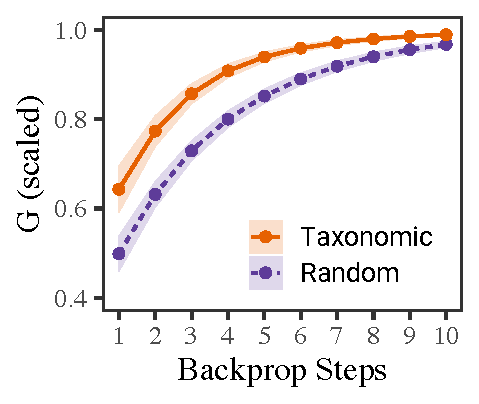
\includegraphics[width=0.5\columnwidth]{robertamammal.pdf}
%     \caption{Scaled generalization scores ($\mathbb{G}$) for mammals }
%     \label{fig:roberta-mammal}
% \end{figure}

% \texttt{log\_prob $\sim$ n + c\_type * sim * overlap}
% We use the adapted models from the previous section and plug them into the induction stage of the framework (Fig. 1B)
% \km{We use our framework to study the extent to which qualitative patterns observed in human induction experiments are also observed when using LMs as the inductive reasoners.}
% \subsection{Premise Monotonicity}
% The phenomena of premise monotonicity suggests that inclusivity of the premise concepts promotes inductive generalization \citep{osherson1990category}. 
% That is, arguments with greater number of premise concepts are generally stronger than those with fewer premise concepts.
% \paragraph{Data generation} We generate data to reflect this phenomena by relying on the taxonomy in our concept data. 
% Specifically, we consider the animal-kingdom subset of the taxonomy and use the top-10 superordinate categories based on number of members (e.g., \textit{mammals, birds,} etc.)
% We use three different novel properties in this experiment, each belonging to a different property domain -- \textit{can dax} (behavioral), \textit{is a dax} (taxonomic), and \textit{has a dax} (visual).
% To simulate monotonicity, we 
% % \km{To simulate monotonicity, we incrementally sample a set of 1,..,7 concepts from each superordinate and use it as the adaptation set, i.e., we create 7 different adaptation sets per superordinate category. The left-over concepts were used as the generalization set. }
% \paragraph{Induction} 

% \km{Results}
% \subsection{Conclusion Specificity}
% The homogeneity of the conclusion concept with respect to the premise concepts affects inductive generalization of novel properties \citep{osherson1990category}. 
% For the same set of premise concepts subsumed by a common superordinate concept (e.g., \textsc{robin}, \textsc{sparrow}), inductive arguments with more specific conclusion concepts (e.g., \textsc{bird}) are stronger than those with more general conclusion concepts (e.g., \textsc{animal}). 
% This implies that more evidence is typically needed to support a conclusion whose concept has greater coverage relative to the premise concepts.

% \km{Data generation}

% \km{Test}

% \km{Results}



\bibliographystyle{apacite}

\setlength{\bibleftmargin}{.125in}
\setlength{\bibindent}{-\bibleftmargin}

\bibliography{CogSci_Template}


\end{document}
